\documentclass[main]{subfiles}
\begin{document}

%@@@@@@@@@@@@@@@@@@@@@@@@@@@@@@
% Main Topics: optimality conditions for convex problems, Newton method
% Convex Optimization and the Newton Method - 02.11.2017
% author: Vanessa Leite

\section{Convex Optimization and the Newton Method}

\emph{$f$ is always a convex function from now on.}

\subsection{Convex optimization}
\paragraph{Basic properties}
$f(x^*) = \displaystyle \min_{x \in Q} f(x)$, $f$ convex function, $Q$ convex
set, $Q \subseteq dom(f)$, $f^*$ is the optimal solution.

\emph{Remember: to identify optimal solutions, we need to evaluate conditions
(in any class of optimization problems).}

\paragraph{Lemma: $f$ continuously differentiable on $dom(f)$. $x^* \in Q$ is a
minimizer $\iff \nabla f(x^*)^T (y-x^*) \geq 0$, $\forall y \in Q$.}

\subparagraph{Proof:}
$x^* \in Q$ satisfies $\nabla f(x^*)^T (y-x^*) \geq 0$, $\forall y \in Q$, then
$f(y) \geq f(x^*) + \nabla f(x^*)^T (y-x^*) \geq f(x^*)$, $\forall y \in Q$.
Conversely, assume $f(x^*) = f^*$ and suppose $\exists y \in Q$ st $\nabla
f(x^*)^T (y-x^*) < 0$.\\
$\phi \mathbb{R} \mapsto \mathbb{R}$, $\phi(\lambda) = f(\lambda y +
(1-\lambda)x^*)$. $\phi$ is convex.\\
$\phi'(\lambda) = \nabla f(\lambda y + (1-\lambda)x^*)$.\\
$\phi'(0) = \nabla f(x^*)^T(y-x^*) \underbrace{< 0}_{\text{by assumption}}$.\\
$\exists \lambda > 0$ such that $\phi)\lambda) < \phi(0)$, this is a
contradiction.

\paragraph{Lemma: $f$ continuously differentiable on $dom(f)$. $x^* \in dom(f)$
attains $f^* \iff \nabla f(x^*) = 0$.}

\subparagraph{Proof:}
if $x^* \in dom(f)$ and $\nabla f(x^*) = 0$, then, $\forall y \in dom(f)$,
$f(y) \geq f(x^*)+ \nabla f(x^*)^T (y-x^*) = f(x^*)$.\\
Conversely, suppose $x^* \in dom(f)$ attains $f^*$. Choose some positive number
$t > 0$ such that $y = x^* - t \nabla f(x^*) \in dom(f)$.\\
From previous lemma, $0 \leq \nabla f(x^*)^T(y-x^*) = -t \underbrace{||\nabla
f(x^*)||^2}_{\rightarrow 0} \leq 0$.

\paragraph{Lemma: Let $f_1, \dots, f_m$: be convex functions.
Let $D = \bigcap^m_{i=1} dom(f_i) \subseteq \R^n$. $f(x) = \max \{f_1(x),
\dots, f_m(x)\}$ $\forall x \in D$ is convex.}

\begin{figure}[!h]
  \label{fig:projection}
  \centering
    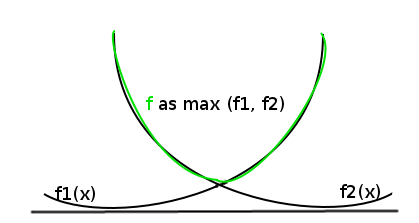
\includegraphics[width=0.3\textwidth]{imgs/max-convex-functions.png}
    \caption{$f$ now is convex, we cannot replace $\max$ with $\min$ because it
    will result in a concave function instead.}
\end{figure}

\subparagraph{Proof:}
$\forall x,y \in D$: $f(\lambda x + (1-\lambda)y)
= \max \{f_i(\lambda x + (1-\lambda) y)$: $i = 1, \dots, m\}
\leq \max \{ \lambda f_i(x) + (1-\lambda)f_i(y)$: $i = 1, \dots, m\}
\leq \max \{\lambda f_i(x)$: $i = 1, \dots, m\} + \max \{(1-\lambda) f_i(y)$:
$i =1, \dots, m\}
= \lambda \max\{f_i(x)$: $i =1, \dots, m\} + (1-\lambda) \max \{f_i(y)$: $i =1,
\dots, m \}
=\lambda f(x) + (1-\lambda f(y)$

\paragraph{Definition: strongly convexity \emph{(not strictly convexity)}}
$f: dom(f) \mapsto \R$ is strongly convex with modulus $\sigma > 0$, if
$\forall \lambda \in (0,1)$ and $x, y \in dom(f)$: $f(\lambda x + (1-\lambda)y)
+ \frac{\sigma}{2} \lambda(1-\lambda) || y - x||^2 \leq \lambda f(x) +
(1-\lambda)f(y)$.

\paragraph{Remark: Let $f$ be continuously differentiable on $dom(f)$.
Then $f$ is strongly convex with modulus $\sigma \iff f(y) \geq f(x) + \nabla
f(x)^T (y-x) + \frac{\sigma}{2} ||y-x||^2$ $\forall x, y \in dom(f)$.
Then, $f$ is strongly convex with modulus $\sigma \iff \nabla^2 f(x)
\geq \sigma I$}
Example: $f(x) = ||x||^2$ is strongly convex with modulus $2$ (diagonal of
Hessian Matrix is $2$.

\paragraph{Remember:}
Hessian Matrix is a square matrix of second order partial derivatives.\\
$H_{ij} = \frac{\partial^2 f}{\partial x_i \partial x_j}$.
Hessian matrix of a convex function is PSD. If Hessian is positive definite at
$x$, then $f$ attains an isolated local minimum at $x$. If it is negative, then
$f$ attains an isolated local maximum. If it has both positive and negative
eigenvalues, then $x$ is a saddle point for $f$.

\paragraph{Lemma: if $f$ is strongly convex and twice differentiable with
modulus $\sigma$, then for all $x \in dom(f)$,
$\nabla^2 f(x)^{-1}$ (inverse of the Hessian) exists and
$||\nabla^2 f(x)^{-1} y||^2 \leq \frac{||y||^2}{ \sigma^2}
\forall y \in dom(f)$.}

\subparagraph{Proof:}
Let $A = \nabla^2 f(x)$ be the Hessian Matrix. $A \geq \sigma I$, $A$ is
symmetric and $A^{-1}$ exists.\\
$\forall y \in dom(f)$: $y^T Ay \geq \sigma ||y||^2$ (from PSD fact)\\
$y^T A^{-1}y = y^T A^{-1}A A^{-1}y \geq \sigma ||A^{-1}y||^2$ (*)\\
$||y||^2 = y^Ty = y^T A^{-\frac{1}{2}}A^{\frac{1}{2}}A^{\frac{1}{2}}
A^{-\frac{1}{2}} y = y^T A^{-\frac{1}{2}} A A^{-\frac{1}{2}}y \geq
\sigma ||A^{-\frac{1}{2}}y||^2$\\
$= \sigma y^T A^{-1}y \underbrace{\geq}_{*} \sigma ||A^{-1}y||^2$.

\subsection{The Newton Method}

$f^* = \displaystyle \min_{x \in dom(f)} f(x)$\\
"no constraints" (convex optimization without constraints)

Assumptions:
\begin{itemize}
\item $f$ is twice differentiable on $dom(f)$
\item $f$ is strongly convex with modulus $\sigma$
\item There exists a constante $L > 0$ such that $||\nabla^2 f(x)
- \nabla^2f(y)||_\nabla \leq L ||x-y||_2$ $\forall x, y \in dom(f)$,
where $||A||_\nabla = sup\{\frac{||Az||_2}{||z||_2}: z \neq 0 \}$
\item $\exists x_0 \in dom(f)$ such that $||\nabla f(x_0)||_2 \leq
\frac{\sigma^2}{L}$
\end{itemize}

Goal: find $x^* \in dom(f)$ such that $\nabla f(x^*) = 0$.
(There are many situation where this is not easy to find.)\\
Develop an iterative scheme:\\

Aapproximate functions: $x \mapsto \nabla f(x_t) + \nabla^2 f(x_t)(x-x_t)$\\
Now, we set this function to be zero:\\
$\nabla f(x_t) + \nabla^2 f(x_t)(x-x_t) = 0 \iff x_{t+1} = x_t + \delta t$.\\
$\delta t = -[\nabla^2 f(x_t)]^{-1} \nabla f(x_t)$\\

\paragraph{Newton Method's Algorithm}

\begin{enumerate}
\item Begin with $x_0$
\item For $0 \leq t \leq T$:
\subitem compute $\delta t = -[\nabla^2 f(x_t)]^{-1} \nabla f(x_t)$ and set
$x_{t+1} = x_t + \delta t$
\item return $x_t$
\end{enumerate}


\paragraph{Theorem: $f(x_t) - f^* \leq \frac{2 \sigma^3}{L^2}
(\frac{1}{2})^(2^{T+1}$}

\subparagraph{Proof:}
We know $f(y) \leq \underbrace{f(x_t) + \nabla f(x_t)^T(y-x_t) +
\frac{\sigma}{2} ||y - x_t||^2}_{= g(y)}$ $\forall y \in dom(f)$.\\
$g(y)$ is strictly convex and attains its minimum at
$y^* = x_t - \frac{1}{\sigma} \nabla f(x_t)$.\\
$\rightarrow f(y) \geq g(y) \geq g(y^*) = f(x_t) - \frac{1}{2 \sigma}
||\nabla f(x_t)||^2$\\
$\rightarrow f^* \geq f(x_t) - \frac{1}{2 \sigma}||\nabla f(x_t)||^2
\rightarrow f(x_t) - f^* \leq \frac{1}{2 \sigma}||\nabla f(x_t)||^2$

$||\nabla f(x_{t+1})|| = ||\nabla f(x_t + \delta t)||$\\
$= ||\nabla f(x_t + \delta t) - \nabla f(x_t) - \nabla^2 f(x_t) \delta t ||$\\
$= || \int_{0}^{1} \nabla^2 f(x_t + s \delta t) \delta t ds - \nabla^2 f(x_t)
\delta t||$\\
$= \int_{0}^{1} ||[ \nabla^2 f(x_t + s \delta t) - \nabla^2 f(x_t) ] \delta t
ds||$\\
$\leq \int_{0}^{1} ||[\nabla^2 f(x_t + s\delta t) - \nabla^2 f(x_t)] \delta t||
ds$\\
$\leq \int_{0}^{1} ||\nabla^2 f(x_t + s\delta t) - \nabla^2 f(x_t)||_\nabla
\times ||\delta t|| ds$\\
$\leq \int_{0}^{1} L \times \underbrace{||x_t + s\delta t - x_t||}_{\text{from
nabla norm}} || \delta t|| ds$\\
$= \int_0^1 L s ||\delta t||^2 ds$ \\
$= \frac{L}{2} || \delta t||^2 = \frac{L}{2} || \underbrace{\nabla^2
f(x_t)^{-1} \nabla f(x_t)}_{\text{definition of $\delta t$}} ||^2$\\
$\underbrace{\leq}_{\text{lemma 3}} \frac{L}{2 \sigma^3} ||\nabla f(x_t)||^2$\\
$\rightarrow f(x_t) - f^* \leq \frac{1}{2 \sigma} ||\nabla f(x_t)||^2 \leq
\frac{2 \sigma^3}{L^2} (\frac{1}{2})^{2^{T+1}}$.


\end{document}
